\chapter{Projektowanie i implementacja}
\label{cha:implementacja}

Nakreślony problem -- rozproszonego systemu, który dzięki propagacji danych między użytkownikami obniży obciążenie serwerów sieci Web -- stawia wiele wyzwań projektowych i architektonicznych.

\section{Wymagania funkcjonalne}
\label{sec:funkcjonalnosc}

System dHTTP, z punktu widzenia użytkownika, ma spełniać jedną funkcjonalność: utrzymać lub poprawić płynność dostępu do interesujących go witryn internetowych, nie wpływając na ich treść i nie naruszając prywatności.

Projekt udostępnia interfejs zapewniający dostęp do statystyk, a także preferencji użytkownika. Udostępnione preferencje dotyczą: stopnia działania aplikacji w tle, trybów propagacji i przechowywania danych.
% To może powinno być gdzieś indziej
\begin{figure}[h]
	\centering
    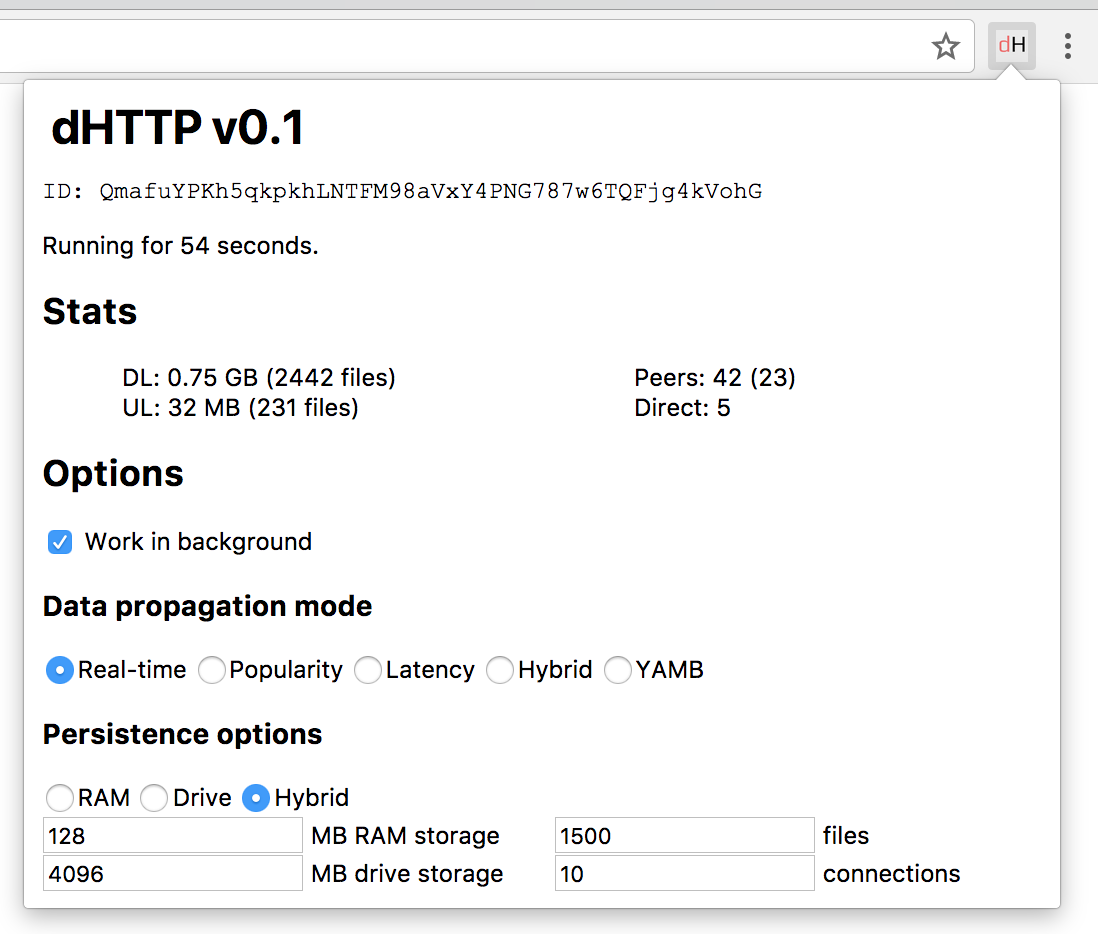
\includegraphics[scale=0.5]{dhttp-initial-interface.png}
	
	\caption{\label{fig:initialInterface} Wstępna implementacja interfejsu operacji dla systemu dHTTP: pop-up dostarczany przez wtyczkę do przeglądarki Google Chrome pozwala na obserwację statystyk i zmianę preferencji.}
\end{figure}

% TODO - gdzieś w pracy podkreśl, jak bardzo istotna jest prosta i automatyczna klastryzacja
Wymogiem dla projektu, koniecznym z racji potrzeby prostej automatyzacji rozrostu sieci, jest tryb niezależny aplikacji -- {\em headless mode} -- pozwalający na wystartowanie niezależnego węzła jednym poleceniem. Niezbędnym jest, aby węzeł tego typu udostępniał statystyki użycia i wstępną konfigurację przy użyciu poleceń interfejsu konsolowego, pozwalając jednak na funkcjonalne uruchomienie z domyślną konfiguracją.


\section{Definicje, architektura i technologie}
\label{sec:zalozeniaProjektu}

\subsection{Słownik pojęć}

W celu uniknięcia niejednoznaczności w dalszym toku pracy, zdefiniowane zostaną następujące pojęcia:

\begin{itemize}
    \item \textbf{węzeł} -- pojedynczy, autonomiczny element systemu, który wykorzystuje komunikację sieciową w celu rozgłaszania i pobierania danych;
    \item \textbf{klient} -- węzeł, który pobiera dane w celach użytkowych, zaimplementowany w wersji dedykowanej użytkownikowi końcowemu;
    \item \textbf{klaster} -- zbiór węzłów, który posiada informacje i ścieżki komunikacyjne pozwalające efektywnie na wymianę informacji pomiędzy każdym z nich;
    \item \textbf{metadane klastra} -- ustrukturyzowane informacje wymieniane pomiędzy węzłami w celu ustalenia stanu i optymalizacji działania klastra;
    \item \textbf{metadane pliku} -- ustrukturyzowane informacje wymieniane między węzłami w celu propagacji i umożliwienia wymiany faktycznych danych plikowych;
\end{itemize}
      % TODO - dodać nowe, jeśli się pojawią/przyjdą do głowy

\subsection{Koncept architektury}

Z punktu widzenia klastra, koncepty węzła i klienta są jednoznaczne i równorzędne -- wszystkie wyposażone są we wspólne mechanizmy komunikacji, i protokół wymiany danych między nimi działa na niezmienionej zasadzie. Wspólnie budować będą rozproszoną tablicę haszującą (DHT), która pozwoli na dostęp do metadanych klastra, które informować będą o cechach poszczególnych węzłów, oraz metadanych plików, przyspieszając proces ich identyfikacji i zapewniając oraz bezpieczeństwo spójność danych.

W celu zapewnienia płynności działania systemu, metadane klastra powinny zawierać w sobie informacje o {\em reputacji} poszczególnych węzłów. Podczas gdy węzły serwerowe z reguły zostają uruchomione i będą działać, mając szczyty obciążenia czy wymagań zależne głównie od obciążenia całej sieci (lub ewentualnego alternatywnego oprogramowania serwerowego na nich uruchamianego), węzły klienckie podlegać będą prawdopodobnie o wiele większej dynamice, z racji licznych odczytów dużych plików i podejścia użytkownika, które może zakładać częste otwieranie i zamykanie przeglądarki.

Węzły serwerowe i klienci powinny mieć zatem różne wartości bazowe przy ocenie ich sprawności w sieci -- reputacja oprogramowania klienckiego powinna być domyślnie niższa, i szybciej reagować na zmiany jej wartości.

\subsection{Wykorzystane technologie i narzędzia}
\label{sec:techNTools}
% akapit poniżej prawdopodobnie jest o wiele lepszą kanwą dla czegoś w części teoretycznej niż czymś, co powinno być tutaj.

Budowa kompletnego stosu technologicznego dla projektu o takich wymaganiach przez lata pozostawała problemem nietrywialnym. Paradygmaty programowania specjalizowane w podejściu obiektowym wspierały budowę monolitów, a komunikacja klient-serwer często polegała na tworzeniu dużej ilości poleceń, bez skupienia na wydajności takich rozwiązań.

Dużą zmianą w tej kwestii jest rozwój \texttt{libp2p}, stanowiący efekt długotrwałej pracy nad zrozumieniem stosu sieciowego Internetu, zbiór protokołów i wyprowadzonych zeń narzędzi, mechanik i interfejsów, pozwalających na ich podstawie budować własne, kompleksowe rozwiązania (\cite{libp2p-specs}).

\texttt{libp2p} stanowi względnie wysokopoziomową kanwę dla projektu dHTTP. To właśnie na efektach pracy tego projektu opiera się warstwa tworzenia i komunikacji węzłów, budująca klaster dHTTP. Implementacja \texttt{js-libp2p} udostępnia moduły niezbędne w komunikacji sieciowej, łączeniu strumieni różnych protokołów, wykrywaniu nowych węzłów, propagowaniu informacji o istniejących węzłach sieci czy wreszcie budowaniu rozproszonej tablicy haszującej, stanowiącej bazę metadanych klastra i plików.

Nie bez wpływu pozostaje rozwój przeglądarek internetowych. Współczesne browsery udostępniają kompleksowe API, pozwalające rozwijać wtyczki zmieniające zawartość stron internetowych, z uwzględnieniem kwestii wydajności i bezpieczeństwa. Istotne jest również wsparcie dla nowych technik komunikacji takich jak {\em WebSockets}, pozwalającej na wymianę informacji w czasie rzeczywistym, dzięki utrzymywaniu dwustronnie interaktywnej sesji TCP pomiędzy przeglądarką i serwerem. W ramach tej pracy rozwinięta została wtyczka dla przeglądarki Google Chrome. Wybór ten podyktowany został znaczną przewagą Chrome -- w chwili pisania tej pracy, udział Chrome w rynku przeglądarek na komputerach osobistych wynosił ponad 64\% (\cite{chromeStats}). Prace i testy przeprowadzono przy użyciu 64-bitowego Google Chrome w wersji 63.0, na platformie macOS w wersji 10.13.2.
% TODO cite https://developer.chrome.com/extensions lub bardziej specyficznie.

Za powstanie {\em headless} dHTTP w znacznej części odpowiada Node.js -- środowisko uruchomieniowe pozwalające na uruchamianie kodu JavaScript po stronie serwerowej.  Narzędzia, takie jak \texttt{npm} i Browserify, pozwalają z kolei na wykorzystywanie serwerowego kodu JavaScriptu w kodzie klienckim. Dzięki możliwości rozwoju obu aplikacji przy użyciu tego samego języka programowania i powyższym rozwiązaniom, znaczna część  kodu aplikacji może być współdzielona. {\em headless} dHTTP testowane było przy użyciu \texttt{node} w wersji v8.9.1, na platformie macOS oraz Amazon Linux AMI.

% Języki programowania nie były zaadaptowane do prostej komunikacji sieciowej, a przeglądarki nie wspierały krytycznych narzędzi i protokołów pozwalających na komunikację w czasie rzeczywistym, pozostawiając problemy natury wydajnościowej uniemożliwiające użyteczną implementację tego typu rozwiązań.

\subsection{Paradygmaty i koncepcje}
Istotą projektu dHTTP jest reagowanie na zapytania i komunikacja pomiędzy węzłami. Ponadto, projekt działać będzie w środowisku JavaScriptowym -- język ten (poza web workers -- rozwiązaniem polegającymi na delegacji obliczeń do wydzielonego środowiska, patrz: \cite{webWorkers}) uruchamiany jest jednowątkowo. W klasycznym podejściu do programowania może to powodować problemy związane z blokowaniem się wydarzeń; jest to dotkliwe zwłaszcza w przypadku interfejsów użytkownika, które w takiej sytuacji tracą responsywność. Poniżej znajduje się omówienie związanym z tych praktyk, które stosowane są w projekcie dHTTP.
% TODO - podkreśl jak pozytywny wpływ ma to wszystko na sposób pisania dHTTP

\subsubsection{Asynchroniczność}
Podstawowym rozwiązaniem stosowanym w języku JavaScript, pozwalającym na wykonanie w środowisku jednowątkowym, jest model współbieżności oparty o tzw {\em event loop}. Wywołania funkcji odkładane są na stosie, podczas gdy kolejne wiadomości są wkładane do kolejki FIFO. Podstawowym założeniem jest nigdy nie blokować -- jeśli jakieś wywołanie wymaga konkretnej reakcji, definiowanej przez użytkownika, należy nasłuchiwać wydarzeń lub użyć wywołań zwrotnych (\texttt{callback}).

\begin{lstlisting}[language=javascript]
    function foo(callback) {
        var a = someWaitingOperation()
        callback(a)
    }

    foo((a) => print(a))
    console.log('Hello, world!')
\end{lstlisting}

W powyższym przykładzie warto zauważyć, że wywołanie \texttt{console.log(...)} będzie miało miejsce natychmiast po zawołaniu funkcji foo -- jest więc bardzo prawdopodobnym, że efekt jego pracy widoczny będzie przed zawołaniem funkcji \texttt{callback}.

Asynchroniczne odwołania są kluczowe w przypadku wydarzeń takich jak oczekiwanie na odpowiedź serwera; czekając na odpowiedź, możemy kontynuować tok życia programu.

\subsubsection{Event-driven architecture}
Pozioma oś modelu współbieżności JavaScriptu zapewnia natywne wsparcie dla reakcji na wydarzenia. W celu nasłuchiwania wydarzenia, zarejestrować jego obserwatora ({\em listener}) stosując z reguły składnię zbliżoną do:
\begin{lstlisting}[language=javascript]
    a.addEventListener('click', ()=> {
        console.log('Button clicked!')
    })
\end{lstlisting}

\begin{figure}[h]

    \centering
    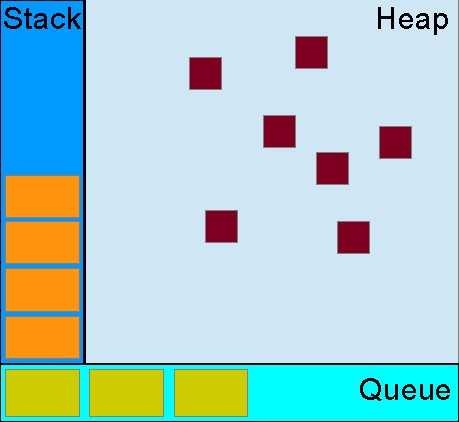
\includegraphics[scale=0.6]{js-concurrency.pdf}
    % \subcaption{\label{subfigure_a}}

	\caption{Wizualizacja modelu współbieżności języka JavaScript -- widać stos funkcji (oś pionowa) i kolejkę wydarzeń (oś pozioma). Pomiędzy nimi znajduje się współdzielona sterta, zapewniająca dostęp do danych. Źródło: \cite{eventLoop}}

\end{figure}

\subsubsection{Strumienie}
% i potoki

Node.js przeniósł języki, którego dotychczasowym targetem były lekkie rozwiązania klienckie, na poziom serwerowy, w którym niektóre operacje są długotrwałe, mają przerwy w wywołaniach i nierzadko wymagają informowania o postępach (przykładem może być utrzymanie połączenia sieciowego, czy odczyt standardowego wyjścia) Choć jest możliwym implementacja tego typu rozwiązań  wywołaniami zwrotnymi, czytelność drastycznie spada.

Z pomocą przychodzą strumienie (\cite{nodeStreamAPI}). Strumienie nakładają abstrakcję, która pozwala intuicyjnie czytać (dla strumieni \texttt{Readable}) wrzucać (w przypadku \texttt{Writable}), a także transformować (\texttt{Transform}) wartości przekazywane w strumieniu.

\begin{lstlisting}[language=javascript]
// Przykład nawiązywania połączenia w metaprotokole dHTTP
dhttpClient.node.dial(peerInfo, '/dhttp/meta/0.1', (err, connStream) => {
    // connStream to przykład strumienia Duplex - pozwala zarówno na zapis, jak i odczyt.
    // zapisz coś do connStream...
    connStream.write("Let's talk")
    // jeśli w strumieniu pojawią się dane, wywołaj callback. Warto zauważyć, że to wywołanie może nastąpić zarówno przed, jak i po zawołaniu write -- zależy od stanu strumienia, który może otrzymywać dane w innych miejscach programu
    connStream.on('data', (data) => {
        callback(JSON.parse(data))
    })
}


// Przykład uruchamiania serwera HTTP dzięki 'http-server'
http.createServer((req, res) => {
    // Przekaż wartość strumienia req strumieniowi request, który następnie zostanie przekazany do res. W efekcie zadziałamy jako najprostsze proxy - otrzymamy dane o oryginalnym zapytaniu, wywołamy je z punktu widzenia serwera, i przekażemy wynik w ramach odpowiedzi.
    req.pipe(request(req.url)).pipe(res)
}).listen(34887)
\end{lstlisting}

Powyższy przykład, stanowiący część kodu dHTTP, pokazuje istotny koncept {\em potoków} (ang. {\em pipe}). Potoki pozwalają łączyć strumienie w sposób analogiczny do strumieni znanych z systemów Uniksowych: odczytane wartości można przekazać kolejnemu strumieniowi, który może zamienić je na inne wartości, aż w końcu zapiszemy wynik pracy w strumieniu odpowiedzi. Tego typu operacje stanowią kanwę przemian stosowanych w dHTTP.

Podkreślić należy również pozytywny wpływ strumieni na wydajność -- ta abstrakcja pozwala operować na plikach przy użyciu buforów w sposób przezroczysty: przykładowo, aby wysłać duży obrazek nie przechowując go w całości w pamięci, wystarczy utworzyć strumień pliku i przepotokować go do strumienia wyjściowego.

\begin{lstlisting}[language=javascript]
    var fileStream =  fs.createReadStream('files/caviar.jpg');
    fileStream.pipe(connStream)
    //kiedy strumień pliku się zakończy, zamknij połączenie aby poinformować odbiorcę, że nic już na niego nie czeka
    fileStream.on('finish', ()=> connStream.close())
\end{lstlisting}



% \subsection{Problemy warstwy sieciowej}
% \label{sec:networkIssues}
% % to w toku implementacji
% Choć przeglądarki implementują coraz więcej rozwiązań i pozwalają na stosowanie najnowszych protokołów, niektóre kwestie pozostają poza ich kompetencjami.

% Największym problemem systemów opartych o IPv4 jest obecnie wyczerpana pula adresów. Protokół, o który wciąż oparta jest większość komunikacji Internetu, wspiera maksymalnie 4~294~967~296 adresów -- co mogło wydawać się gigantyczną liczbą w momencie implementacji, szybko jednak zostało pochłonięte przez sieć.

% W celu walki z zaimplementowano wiele rozwiązań, od 

% Jak Bóg da, to się napisze te rzeczy
% \subsubsection{Decentralizacja czy rozproszenie?}
% \label{sec:decentralizacjaCzyRozproszenie}

% \subsection{Bezpieczeństwo}
% \label{sec:security}

% \subsubsection{Czy autentykacja to nasza brożka?}
% \subsubsection{Gdzie leżą granice zdrowych heurystyk?}

% \subsection{Enkapsulacja}

% \subsection{Komunikacja}

% Z tego poniżej może powstać osobny rozdział, gdzie to co powyżej stanowiłoby bardziej rozważania na temat właściwego podejścia do realizacji projektu, a to poniżej -- faktyczny opis implementacji systemu, podzielony bardziej granularnie dla każdego z elemenetów

\section{Interfejs \texttt{dhttp.js}}

Podstawę logiki systemu stanowi plik \texttt{dhttp.js}. Jest on interfejsem łączącym backend i stronę użytkową, pozwalającym na dostęp do informacji na temat sposobu działania węzła, a także wykonywanie operacji w sieci dHTTP.

\texttt{dhttp.js} operuje na dwóch protokołach:

\begin{itemize}
    \item \texttt{/dhttp/meta/0.1} -- {\em metaprotokół}, stanowi podstawę szkieletu systemu dHTTP. Informuje o dostępnych węzłach i plikach, obciążeniu sieci, a także następujących na bieżąco zmianach. Konwencją podjętą dla {\em metaprotokołu} jest powszechna propagacja danych -- przykładowo, jeśli łączę się z nowym węzłem, powinienem wysłać mu listę posiadanych przeze mnie plików, a jeśli planuję opuścić sieć, powinienem poinformować o tym wszystkich podłączonych sąsiadów. Dzięki temu podejściu każdy węzeł posiada zbiór informacji na temat otoczenia, pozwalający na szybsze podejmowanie decyzji.

    \item \texttt{/dhttp/data/0.1} -- {\em protokół danych}, stanowi system przesyłu docelowych plików w dHTTP. Zorientowany strumieniowo, przesyła zgromadzone pliki w ich oryginalnym formacie. Może zostać rozszerzony o obsługę zapytań cząstkowych -- tak, aby duże pliki pobierać częściami od swoich sąsiadów.
\end{itemize}
Ponadto, \texttt{dhttp.js} wykorzystuje wbudowane mechanizmy \texttt{libp2p} w celu wykrywania sąsiadów i zmian sieci.
% tutaj bardzo duże wypisanie wszystkich szczegółów jakie dają protokoły, z rysunkami i wszyściutkim

\section{Aplikacje}

\subsection{Węzeł}

\subsection{Przechowywanie danych}
\label{sec:dataPropagation}

\subsection{Klient}



